%% LyX 1.1 created this file.  For more info, see http://www.lyx.org/.
%% Do not edit unless you really know what you are doing.
\documentclass[prb,aps,twocolumn]{revtex4}

\usepackage{graphicx}
\usepackage{amsfonts}
\usepackage{amsmath}
\usepackage{bm}
\usepackage{alltt}
\usepackage{dcolumn} 
\usepackage{amsmath} 
\usepackage{graphicx}
\makeatletter 
\makeatother

\begin{document}

\title{\textbf{Arcurate Computation of the Interation Tensor in Periodic Systems}}


\author{C.J. Tymczak}
\author{Matt Challacombe}

\affiliation{Theoretical Division, Los Alamos National Laboratory, Los Alamos,
New Mexico 87545 }

\date{\today}

\begin{abstract}

\end{abstract}

\maketitle

\section{INTRODUCTION}

When simulating bulk behavior in solids or liquids, Periodic Boundary
Conditions (PBC) are often essential to employ \cite{Allen90}. Therefore,
we have implemented Periodic boundary conditions into the linear scaling
Quantum Chemistry code \textbf{MondoSCF} 
\cite{Challacombe96,Challacombe97,Challacombe99}.
For the two-electron Coulomb matrix, we achieve this via an exact multipole expansion 
of the long range Coulomb field \cite{White94,Challacombe97b}. This yields a spherically
summed boundary condition that is easily transformed to Ewald boundary
condition \cite{Redlack72,Redlack75}.


\subsubsection{The Periodic Far Field Coulomb matrix}

To obtain the periodic far field correction to the matrix elements
we replace the integral in equation (\ref{Jpff}) with the multipole
sum \cite{Challacombe97}
%
\begin{eqnarray}
J_{ab}^{PFF} &=& \frac{1}{2}\sum _{{\mathbf{R}'}\in V_{\infty }-V_{in}}\, \int _{V_{\infty }}
\, d{\mathbf{x}}\, d{\mathbf{x}'}\frac{\rho _{ab}^{loc}\left( {\mathbf{x}}\right) \: \rho ^{loc}
\left( {\mathbf{x}'+\mathbf{R}'}\right) }{\left| \mathbf{x}-\mathbf{x}'\right| } 
\nonumber\\
&=& \frac{1}{2}\sum _{{\mathbf{R}}\in V_{\infty }-V_{in}}\, \sum _{l=0}^{L}\, 
\sum _{l'=0}^{L'}\, \sum _{m=-l}^{l}\, \sum _{m'=-l'}^{l'}
\nonumber\\
 & & \left( -1\right) ^{l}\, {\cal O}_{l}^{m}[\rho _{ab}^{loc};\mathbf{R}_{0}]
\, M_{l+l'}^{m+m'}[\mathbf{R}]\, {\cal O}_{l'}^{m'}[\rho ^{loc};\mathbf{R}_{0}]
\nonumber\\
& &\label{Jpff_2} 
\end{eqnarray}
%
where \( \mathbf{R}_{0} \) is an arbitrary point in the simulation
cell (usually the center of the cell). Let us define
\begin{equation}
\label{ScriptM}
{\cal M}_{l}^{m}=\sum _{{\mathbf{R}'}\in V_{\infty }-V_{in}}\, M_{l}^{m}[\mathbf{R}]
\end{equation}
Which allow us to rewrite
%
\begin{eqnarray}
J_{ab}^{PFF} &=&\frac{1}{2}\sum _{l=0}^{L}\, \sum _{l'=0}^{L'}\, \sum _{m=-l}^{l}\, \sum _{m'=-l'}^{l'}
\nonumber\\
& & \left( -1\right) ^{l}\, {\cal O}_{l}^{m}[\rho _{ab}^{loc};\mathbf{R}_{0}]\,
 {\cal M}_{l+l'}^{m+m'}\, {\cal O}_{l'}^{m'}[\rho ^{loc};\mathbf{R}_{0}]
\nonumber\\
\label{sp_jpff_2}
\end{eqnarray}
%
For \( l=1 \) and \( 2 \) equation (\ref{ScriptM}) is a conditional
summation. In Appendix C we describe an efficient method which allow
us calculate these conditional summations. The only task remaining
is to determine the region of the inner box summation or the multipole
order \( L \) which we have to expand to. Using equation (\ref{B30})
from Appendix B we obtain for the error bound
\begin{equation}
\label{Rmax}
\tau \leq \frac{C_{\rho }\left| \mathbf{d}_{max}\right| ^{L+1}}{\left| \mathbf{R}_{max}
\right| ^{L+1}\left| \left| \mathbf{R}_{max}\right| -2\left| \mathbf{d}_{max}\right| \right| }
\end{equation}
where we are assuming a \( l_{0}=0 \) distribution of unit weight,
and \( \mathbf{R}_{max} \) is the distance to the nearest cell in
the sum in equation (\ref{ScriptM}). 

\section{CONCLUSIONS}

\section*{ACKNOWLEDGMENTS}

We would like to acknowledge Tommy Sewell and Ed Kober for there advise
and support. 

\bibliographystyle{plain}
\bibliography{GaussianPapers}


\appendix

\section{Computation of the \protect\( {\cal M}\protect \) Tensor}\label{calM}

Following the work of Nijboer-De Wette \cite{Nijboer57,Nijboer58a}.
We start by first partitioning  

\begin{equation}
\label{C1}
\frac{1}{r^{l+1}}={\cal G}_{l}\left( \beta ,r\right) +{\cal F}_{l}\left( \beta ,r\right) 
\end{equation}
where

\begin{equation}
\label{C2}
{\cal G}_{l}\left( \beta ,r\right) =\frac{\Gamma \left( l+\frac{1}{2},\beta ^{2}r^{2}\right) }
{\Gamma \left( l+\frac{1}{2}\right) \, r^{l+1}}
\end{equation}
\begin{equation}
\label{C3}
{\cal F}_{l}\left( \beta ,r\right) =\frac{\gamma \left( l+\frac{1}{2},\beta ^{2}r^{2}\right) }
{\Gamma \left( l+\frac{1}{2}\right) \, r^{l+1}}=\frac{\Gamma \left( l+\frac{1}{2}\right) -\Gamma 
\left( l+\frac{1}{2},\beta ^{2}r^{2}\right) }{\Gamma \left( l+\frac{1}{2}\right) \, r^{l+1}}
\end{equation}
where \( \beta  \) is a parameter which controls the convergence.
This allows the lattice sum to be partitioned into rapidly convergent
real and reciprocal space terms 
%
%
\begin{eqnarray}
{\cal M}^{m}_{l} & = & \sum _{\mathbf{R}'\in V_{out}}\, M_{l}^{m}[\mathbf{R}]
\nonumber\\
 & = & \sum _{\mathbf{R}'\in V_{out}}\widetilde{P}_{l}^{m}\left( \cos \theta _{\mathbf{R}}
\right) e^{im\phi _{\mathbf{R}}}\,  {\cal G}_{l}\left( \beta ,\left| \mathbf{R}\right| \right)
\nonumber\\
 & + & \sum _{\mathbf{R}'\in V_{out}}\widetilde{P}_{l}^{m}\left( \cos \theta _{\mathbf{R}}
\right) e^{im\phi _{\mathbf{R}}}\, 
{\cal F}_{l}\left( \beta ,\left| \mathbf{R}\right| \right)
\nonumber\\
&=&\sum _{\mathbf{R}'\in V_{out}}\, \widetilde{P}_{l}^{m}
\left( \cos \theta _{\mathbf{R}}\right) e^{im\phi _{\mathbf{R}}}\, {\cal G}_{l}\left( \beta ,\left|
 \mathbf{R}\right| \right) 
\nonumber\\
&-&\sum _{\mathbf{R}'\in V_{in}}\widetilde{P}_{l}^{m}\left( \cos 
\theta _{\mathbf{R}}\right) e^{im\phi _{\mathbf{R}}}{\cal F}_{l}\left( \beta ,\left| \mathbf{R}\right| 
\right) 
\nonumber\\
&+&\frac{4\pi ^{\frac{3}{2}}(\frac{i}{2})^{l}}{V_{cell}\Gamma \left( l+\frac{1}{2}\right) }
\nonumber\\
&&\sum _{\mathbf{G}\neq \left\{ \emptyset \right\} }\, \left| \mathbf{G}\right| ^{l-2}e^{-\frac{\pi ^{2}\left|
 \mathbf{G}\right| ^{2}}{\beta ^{2}}}\widetilde{P_{l}}^{m}\left( \cos \theta _{\mathbf{G}}
\right) e^{im\phi _{\mathbf{G}}}
\nonumber\\
\label{C4}
\end{eqnarray}
With an appropriate choice of \( \beta \sim \sqrt{\pi }/\left( V_{cell}\right) ^{\frac{1}{3}} \)
the periodic multipole interaction tensor can be computed. The only
potential problem is the computation of the incomplete gamma functions.
Previous approaches attempted to compute this function by the upward
recurrence relation

\begin{equation}
\label{C5}
\Gamma \left( m+1,\, x\right) =m\Gamma \left( m,\, x\right) +x^{m}e^{-x}
\end{equation}
which is started by

\begin{equation}
\label{erfc}
\Gamma \left( \frac{1}{2},\, x\right) =\sqrt{\pi }\, {\rm erfc}\left( \sqrt{x}\right) 
\end{equation}
however, this leads a numerical instability in the calculation. For
large values of \( x \) and \( m \) the calculation of the gamma
function can quickly lose precision. We can remove this problem by
analytically summing the gamma function, collecting terms, and then
rewriting the gamma function as
\begin{eqnarray}
\Gamma \left( m+\frac{1}{2},\, x\right) =\Gamma \left( m+\frac{1}{2}\right) 
\qquad\qquad\qquad
\nonumber\\
\left\{ {\rm erfc}\left( \sqrt{x}\right) 
+\sqrt{\frac{x}{\pi }}\sum _{n=0}^{m-1}(S_{n}\, x\, e^{-\frac{x}{n}})^{n} \right\}
\label{C7}
\end{eqnarray}
where

\begin{equation}
\label{SN}
S_{n}=\left( \frac{\Gamma \left( \frac{1}{2}\right) }{\Gamma \left( n+\frac{3}{2}\right) }
\right) ^{\frac{1}{max(n,1)}}
\end{equation}
Which are tabulated beforehand. We find that this version of the gamma
function is both easy to program and numerically very precise, even
at large \( x \) or \( m \). Table \ref{table:CubicMlm} shows the
matrix coefficients calculated for different cell shapes. We have
also computed the \( {\cal M} \) tensor in one and two dimensions.
The \( {\cal M} \) tensor in one dimension can be computed analytically
%
\begin{eqnarray}
{\cal M}^{m}_{l} & = & \sum _{{\mathbf{R}'}\in V_{out}}\, M_{l}^{m}[\mathbf{R}]
\nonumber\\
& = & \sum _{{\mathbf{R}'}\in V_{out}}\, \widetilde{P}_{l}^{m}\left( \cos \left( 
\theta _{\mathbf{R}}\right) \right) e^{im\phi _{\mathbf{R}}}\, \left\{ \frac{1}{r^{l+1}}\right\} 
\nonumber\\
& = & 
\frac{\widetilde{P}_{l}^{m}\left( \cos \left( \theta _{0}\right) \right) e^{im\phi _{0}}}{a_{0}^{l+1}}
\sum _{n=n_{0}}^{\infty }\frac{1}{n^{l+1}}
\nonumber\\
&+&\frac{\widetilde{P}_{l}^{m}\left( \cos \left( \theta _{0}+\frac{\pi }{2}\right) \right) 
e^{im\left( \phi _{0}+\pi \right) }}{a_{0}^{l+1}}
\sum _{n=n_{0}}^{\infty }\frac{1}{n^{l+1}}
\nonumber\\
& = & Q_{l}^{m}\left[ a_{0},\theta _{0},\phi _{0}\right] \left\{ \zeta (l+1)-
\sum _{n=1}^{n_{0}-1}\frac{1}{n^{l+1}}
\right\}
\nonumber\\
\label{C9}
\end{eqnarray}
%
where \( a_{0} \), \( \theta _{0} \) and \( \phi _{0} \) are the
initial box dimension and angles which are independent of the summation.
In two dimension, the Fourier integrals for the calculation of \( {\cal M} \)
tensor become a lot more complicated, therefore we have chosen to
use the three dimensional formula's and obtain the two dimensional
moments via numerical integration, where we take the limit as the
non-periodic direction goes to infinity,

\begin{eqnarray}
{\cal M}^{m}_{l} & = & \sum _{{\mathbf{R}'}\in V_{out}}\, \left( l-m\right) !\, P_{l}^{m}
\left( \cos \left( \theta _{\mathbf{R}}\right) \right) e^{im\phi _{\mathbf{R}}}\, {\cal G}_{l}
\left( \beta ,\left| \mathbf{R}\right| \right) 
\nonumber\\
 & - & \sum _{{\mathbf{R}'}\in V_{in}}\, \left( l-m\right) !\, P_{l}^{m}\left( \cos \left( 
\theta _{\mathbf{R}}\right) \right) e^{im\phi _{\mathbf{R}}}{\cal F}_{l}\left( \beta ,\left| 
\mathbf{R}\right| \right) 
\nonumber\\
& + &  {\cal C}_1 \sum _{\mathbf{G}\neq \left\{ \emptyset \right\} }\, \left| \mathbf{G}\right| ^{l-2}
e^{-\frac{\pi ^{2}\left|
 \mathbf{G}\right| ^{2}}{\beta ^{2}}}\, {\tilde P}_{l}^{m}\left( \cos \left( \theta _{\mathbf{G}}
\right) \right) e^{im\phi _{\mathbf{G}}}
\nonumber\\
 & = & \sum _{{\mathbf{R}'}\in V_{out}}\, \left( l-m\right) !\, P_{l}^{m}\left( \cos 
\left( \theta _{\mathbf{R}}\right) \right) e^{im\phi _{\mathbf{R}}}\, {\cal G}_{l}\left( \beta ,\left| 
\mathbf{R}\right| \right) 
\nonumber\\
 & - & \sum _{{\mathbf{R}'}\in V_{in}}\, \left( l-m\right) !\, P_{l}^{m}\left( \cos \left( \theta _{
\mathbf{R}}\right) \right) e^{im\phi _{\mathbf{R}}}{\cal F}_{l}\left( \beta ,\left| \mathbf{R}\right| \right)
\nonumber\\
 & + & {\cal C}_2 \sum _{\mathbf{G}\neq \left\{ \emptyset \right\} }\, \int _{-\infty }^{\infty }
\: dG_{z}\: \left| \mathbf{G}
\right| ^{l-2}e^{-\frac{\pi ^{2}\left| \mathbf{G}\right| ^{2}}{\beta ^{2}}}\, 
\nonumber\\
&& \qquad \qquad \qquad \qquad  {\tilde P}_{l}^{m}
\left( \cos \left( \theta _{\mathbf{G}}\right) \right) e^{im\phi _{\mathbf{G}}}
\nonumber\\
\label{C10}
\end{eqnarray}
%
where,
\begin{eqnarray}
{\cal C}_1 = \frac{4\pi ^{\frac{3}{2}}(\frac{i}{2})^{l}}{V_{cell}\Gamma \left( l+\frac{1}{2}\right) }
\nonumber\\
{\cal C}_2 =  \frac{4\pi ^{\frac{3}{2}}(\frac{i}{2})^{l}}{A_{cell}\Gamma \left( l+\frac{1}{2}\right) }
\label{C10p}
\end{eqnarray}
and \( A_{cell} \) is the area of the cell along the non-periodic
direction. We have found that we can obtain the \( {\cal M} \) tensor
matrix elements to 8-10 digits of accuracy with this technique.


\eject


\begin{table*}

\caption{\label{table:CubicMlm} \protect\( {\cal M}_{l}^{m}\protect \) for
a cubic simulation cell \protect\( \left\{ \left| a\right| =1,\left| b\right| =1,\left| c\right| =1,\alpha =\frac{\pi }{2},\beta =\frac{\pi }{2}\right\} \protect \)
and an orthorhombic simulation cell \protect\( \left\{ \left| a\right| =1,\left| b\right| =1,\left| c\right| =1,\alpha =\frac{2\pi }{3},\beta =\frac{2\pi }{3}\right\} \protect \)
where the central cell is subtracted.}

\vspace{0.3cm}
{\centering \begin{tabular}{|c|c|c||c|c|c|}
\hline 
\multicolumn{2}{|c|}{}&
Cubic &
\multicolumn{2}{c|}{ }&
Ortho-rombic\\
\hline
\( \: \:  \)\( l \)\( \: \:  \)&
\( \:  \)\( m \)\( \:  \)&
\( \qquad \qquad  \)\( \quad  \)\( {\cal M}^{m}_{l} \)\( \qquad  \)\( \qquad  \)\( \quad  \)&
\( \: \:  \)\( l \)\( \: \:  \)&
\( \:  \)\( m \)\( \:  \)&
\( \qquad  \)\( \qquad  \)\( \quad  \)\( {\cal M}^{m}_{l} \)\( \qquad  \)\( \qquad  \)\( \quad  \)\\
\hline
4&
0&
0.3095492436410130D+01&
4&
0&
0.8832776225626217D+00 \\
&
4&
0.1547746218205053D+02&
&
3&
0.3122857982921809D+01 \\
\hline 
6&
0&
0.4796724494609411D+01&
6&
0&
-0.3501580359498343D+02\\
&
4&
-0.3357707146226664D+02&
&
3&
0.4332984629874099D+02\\
&
&
&
&
6&
-0.6740542192034350D+03\\
\hline 
8&
0&
0.4276164638449980D+03&
8&
0&
0.1394780314659910D+03\\
&
4&
0.4276164638450001D+03 &
&
3&
0.4931293093807656D+03\\
&
8&
0.2779507014992490D+05 &
&
6&
0.4931293093807656D+03\\
\hline 
10&
0&
0.3337055302939225D+04&
10&
0&
0.1760026471909184D+03\\
&
4&
-0.7341521666466320D+04&
&
3&
0.3422448296725441D+02\\
&
8&
-0.1248058683299270D+06&
&
6&
-0.5324080077525265D+03\\
&
&
&
&
9&
0.1105450799842411D+05\\
\hline 
12&
0&
0.3533770670774835D+06&
12&
0&
0.3441656356582020D+06\\
&
4&
0.2089749967040276D+06&
&
3&
-0.2988963294769746D+06\\
&
8&
0.2086201911558935D+07&
&
6&
0.1981829408275373D+07\\
&
12&
0.3193240788535041D+09&
&
9&
0.1399645778709430D+07\\
&
&
&
&
12&
0.4855992637030970D+09\\
\hline 
14&
0&
0.7186127463179821D+07&
14&
0&
-0.1057046901404442D+08\\
&
4&
-0.9239306738374122D+07&
&
3&
-0.1094473082593862D+08\\
&
8&
-0.5851560934303580D+08 &
&
6&
0.7172818259530190D+07\\
&
12&
-0.2243098358149698D+10&
&
9&
0.1166548139252476D+09\\
&
&
&
&
12&
-0.3299496399383880D+10\\
\hline 
16&
0&
0.1168988444587698D+10&
16&
0&
-0.1553204312146170D+09\\
&
4&
0.5469289478144757D+09&
&
3&
0.2790914628186657D+09\\
&
8&
0.2661931236843469D+10&
&
6&
0.1592904788101633D+10\\
&
12&
0.5130698388451003D+11&
&
9&
0.9241099613788853D+10\\
&
16&
0.1540161278003348D+14 &
&
12&
0.8723232135625955D+11 \\
&
&
&
&
15&
0.3299919999077370D+10\\
\hline
\end{tabular}\par}
\vspace{0.3cm}
\end{table*}


\eject


\begin{figure*}

\caption{\label{figure: SimCell} Simulation cell and interior region.}

{\centering 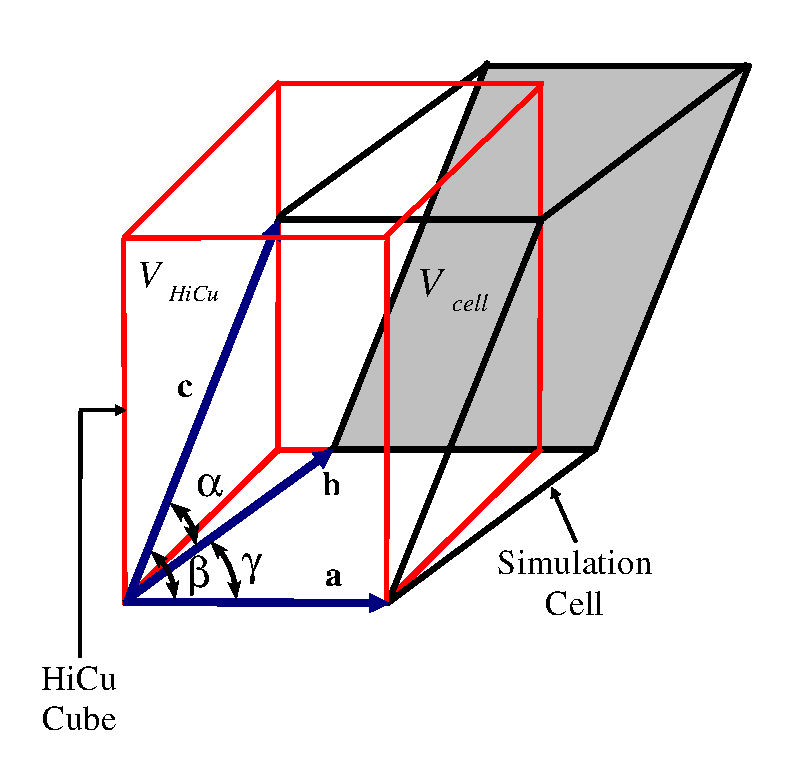
\includegraphics{UnitCell.eps} \par}
\end{figure*}



\begin{figure*}

\caption{\label{figure:ReplicateCells} Regions which contribute to the Coulomb
Matrix}

{\centering 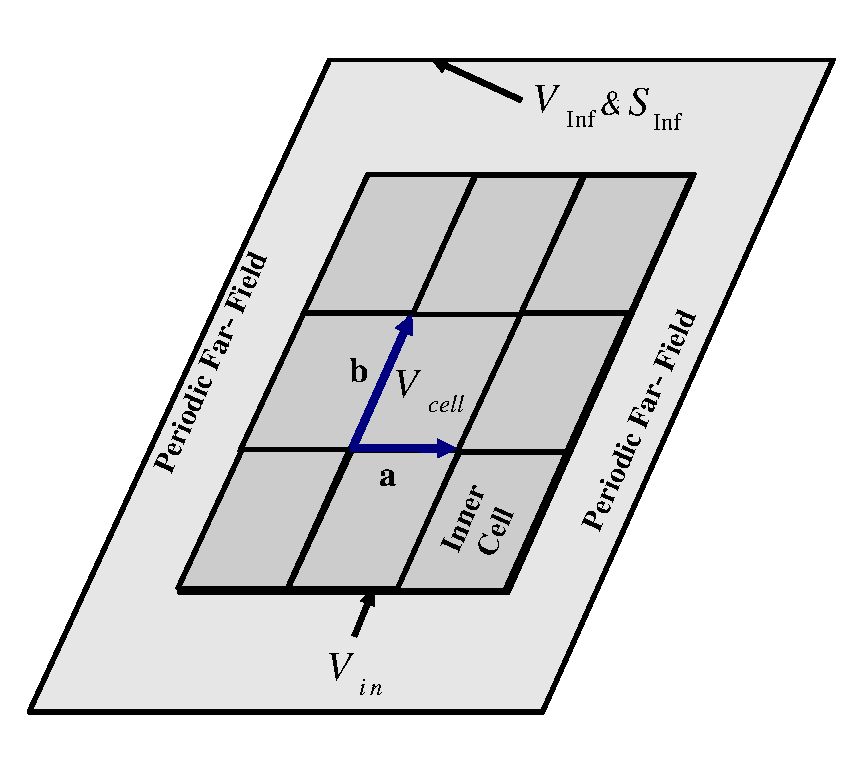
\includegraphics{RepCell.eps} \par}
\end{figure*}



\begin{figure*}

\caption{\label{figure: ErrorPFF} Error in the Periodic Far Field approximation
with increasing \protect\( \mathbf{L}_{max}\protect \) for two different
inner cell sums for \protect\( 64\protect \) molecules of water.}

{\centering \includegraphics{PFFMultipoles_water.ps} \par}
\end{figure*}


\end{document}
